\documentclass[11pt,a4paper]{article}
%%%%%%%%%%%%%%%%%%%%%%%%% Credit %%%%%%%%%%%%%%%%%%%%%%%%

% template ini dibuat oleh martin.manullang@if.itera.ac.id untuk dipergunakan oleh seluruh sivitas akademik itera.

%%%%%%%%%%%%%%%%%%%%%%%%% PACKAGE starts HERE %%%%%%%%%%%%%%%%%%%%%%%%
\usepackage{lmodern}
\usepackage{graphicx}
\usepackage{caption}
\usepackage{microtype}
\captionsetup[figure]{name=Gambar}
\usepackage{tabulary}
\usepackage{minted}
\usepackage{float}
% \usepackage{amsmath}
\usepackage{fancyhdr}
% \usepackage{amssymb}
% \usepackage{amsthm}
\usepackage{placeins}
% \usepackage{amsfonts}
\usepackage[all]{xy}
\usepackage{tikz}
\usepackage{verbatim}
\usepackage[left=2cm,right=2cm,top=3cm,bottom=2.5cm]{geometry}
\usepackage{hyperref}
\hypersetup{
    colorlinks,
    linkcolor={red!50!black},
    citecolor={blue!50!black},
    urlcolor={blue!80!black}
}
\usepackage{subcaption}
\usepackage{multirow}
\usepackage{psfrag}
\usepackage[T1]{fontenc}
\usepackage[scaled]{beramono}
% Enable inserting code into the document
\usepackage{listings}
\usepackage{chngcntr}
\usepackage{xcolor} 
% custom color & style for listing
\definecolor{codegreen}{rgb}{0,0.6,0}
\definecolor{codegray}{rgb}{0.5,0.5,0.5}
\definecolor{codepurple}{rgb}{0.58,0,0.82}
\definecolor{backcolour}{rgb}{0.95,0.95,0.92}
\definecolor{LightGray}{gray}{0.9}
\lstdefinestyle{mystyle}{
	backgroundcolor=\color{backcolour},   
	commentstyle=\color{green},
	keywordstyle=\color{codegreen},
	numberstyle=\tiny\color{codegray},
	stringstyle=\color{codepurple},
	basicstyle=\ttfamily\footnotesize,
	breakatwhitespace=false,         
	breaklines=true,                 
	captionpos=b,                    
	keepspaces=true,                 
	numbers=left,                    
	numbersep=5pt,                  
	showspaces=false,                
	showstringspaces=false,
	showtabs=false,                  
	tabsize=2
}
\lstset{style=mystyle}
\renewcommand{\lstlistingname}{Kode}
%%%%%%%%%%%%%%%%%%%%%%%%% PACKAGE ends HERE %%%%%%%%%%%%%%%%%%%%%%%%


%%%%%%%%%%%%%%%%%%%%%%%%% Data Diri %%%%%%%%%%%%%%%%%%%%%%%%
\newcommand{\studentA}{\textbf{Handayani(122140166)}}
\newcommand{\studentB}{\textbf{Francois Novalentino Sinurat (121140007)}}
\newcommand{\studentC}{\textbf{⁠Dimas Azi Rajab Aizar (121140135)}}
\newcommand{\course}{\textbf{Sistem/Teknologi Multimedia (IF4021)}}
\newcommand{\assignment}{\textbf{Tugas Besar}}
\newcommand{\tanggal}{\textbf{31-05-2025}}

%%%%%%%%%%%%%%%%%%% using theorem style %%%%%%%%%%%%%%%%%%%%
\newtheorem{thm}{Theorem}
\newtheorem{lem}[thm]{Lemma}
\newtheorem{defn}[thm]{Definition}
\newtheorem{exa}[thm]{Example}
\newtheorem{rem}[thm]{Remark}
\newtheorem{coro}[thm]{Corollary}
\newtheorem{quest}{Question}[section]
%%%%%%%%%%%%%%%%%%%%%%%%%%%%%%%%%%%%%%%%
\usepackage{lipsum}%% a garbage package you don't need except to create examples.
\usepackage{fancyhdr}
\pagestyle{fancy}
\lhead{\small Handayani (122140166), Francois Novalentino Sinurat (121140007), Dimas Azi Rajab Aizar (121140135)}
\rhead{ \thepage}
\cfoot{\textbf{SuperPower Menggunakan MediaPipe dan OpenCV}}
\renewcommand{\headrulewidth}{0.4pt}
\renewcommand{\footrulewidth}{0.4pt}

%%%%%%%%%%%%%%  Shortcut for usual set of numbers  %%%%%%%%%%%

\newcommand{\N}{\mathbb{N}}
\newcommand{\Z}{\mathbb{Z}}
\newcommand{\Q}{\mathbb{Q}}
\newcommand{\R}{\mathbb{R}}
\newcommand{\C}{\mathbb{C}}
\setlength\headheight{14pt}

%%%%%%%%%%%%%%%%%%%%%%%%%%%%%%%%%%%%%%%%%%%%%%%%%%%%%%%555
\begin{document}
\thispagestyle{empty}
\begin{center}
	
\includegraphics[scale = 0.15]{Figure/ifitera-header.png}
	\vspace{0.1cm}
\end{center}
\noindent
\rule{17cm}{0.2cm}\\[0.3cm]
Anggota 1: \studentA \hfill Tugas Ke: \assignment\\[0.1cm]
Anggota 2: \studentB \hfill Tanggal: \tanggal\\[0.1cm]
Anggota 3: \studentC \\[0.1cm]
Mata Kuliah: \course \\[0.1cm]
\rule{17cm}{0.05cm}
\vspace{0.1cm}

%%%%%%%%%%%%%%%%%%%%%%%%%%%%%%%%%%%%%%%%%%%%% BODY DOCUMENT %%%%%%%%%%%%%%%%%%%%%%%%%%%%%%%%%%%%%%%%%%%%%


\section*{SuperPower Menggunakan MediaPipe dan OpenCV}

\counterwithin{lstlisting}{section}
\counterwithin{figure}{section}
\counterwithin{table}{section}

\section{Pendahuluan}
Teknologi computer vision dan gesture recognition memainkan peran penting dalam menciptakan interaksi manusia-komputer yang lebih alami dan intuitif, dengan deteksi gerakan tangan real-time sebagai elemen kunci untuk interaksi yang dinamis 
 \cite{martinez2025improved}. Pustaka MediaPipe Python yang terintegrasi dengan OpenCV memungkinkan pelacakan hingga 21 titik penting (landmarks) pada tangan secara efisien, dan telah digunakan dalam berbagai aplikasi seperti kontrol permainan rehabilitasi (exergame), interaksi virtual, serta analisis pose untuk pengenalan emosi \cite{husna2025investigation}. Proyek ini kami bangun dengan tema kekuatan super, lebih tepatnya “SuperPower”, memanfaatkan kombinasi MediaPipe dan OpenCV untuk menciptakan interaksi visual berbasis gestur tangan. Sistem ini mendeteksi gerakan jari pengguna dan memberikan efek animasi seperti api atau partikel yang mengikuti gerakan tangan secara dinamis. Efek-efek ini tidak hanya meningkatkan daya tarik visual, tetapi juga memungkinkan pengalaman pengguna yang lebih immersif dan menyenangkan, menyerupai penggunaan "kekuatan super". Penggunaan pendekatan ini sejalan berbagai konteks interaktif, termasuk game edukatif, pelatihan virtual, hingga terapi rehabilitatif yang mendukung pengembangan antarmuka digital yang lebih menarik, responsif, dan meminimalkan beban pengguna \cite{nuralin2024realtime}.
    
\section{Alat dan Cara Kerja}
Filter ini dibuat menggunakan bahasa pemrograman Python dengan memanfaatkan beberapa library utama yaitu OpenCV untuk pengolahan dan penampilan citra video, MediaPipe untuk deteksi dan pelacakan tangan secara real-time, NumPy untuk manipulasi data numerik, serta ImageIO dan os untuk membaca file animasi dari sistem. Perangkat keras yang digunakan adalah kamera (webcam) yang berfungsi sebagai input untuk menangkap gerakan tangan pengguna. Sedangkan perangkat lunak yang diperlukan mencakup sistem operasi komputer,dan Visual Studio Code. Program ini bekerja dengan menangkap video dari kamera, kemudian menggunakan MediaPipe untuk mendeteksi posisi tangan dan jari. Efek animasi dari file .gif atau .mp4 kemudian ditambahkan secara dinamis ke posisi tangan atau ujung jari yang terangkat. Hasil akhirnya ditampilkan secara langsung dalam jendela video, menciptakan pengalaman interaktif berbasis augmented reality.
    
Proses dimulai dengan pengambilan gambar secara real-time menggunakan kamera, kemudian gambar diproses dan dianalisis menggunakan model deteksi telapak tangan untuk menemukan posisi tangan dalam frame. Setelah posisi telapak tangan teridentifikasi, sistem melanjutkan dengan mendeteksi 21 landmark tangan yang mencakup sendi dan ujung jari. Deteksi ini bersifat 3D dan sangat presisi, sehingga memungkinkan pelacakan gerakan tangan secara detail dan real-time.

Dalam implementasinya pada program, hasil dari deteksi landmark tangan digunakan untuk menentukan posisi yang tepat untuk menempatkan efek visual GIF ke dalam video. Misalnya, jika hanya satu jari yang diangkat, efek akan diarahkan ke ujung jari tersebut. Proses ini didukung oleh pemrosesan gambar dengan OpenCV dan penggunaan MediaPipe untuk pelacakan tangan. Integrasi ini menciptakan pengalaman augmented reality yang responsif dan interaktif, di mana pengguna dapat mengendalikan posisi efek hanya dengan gerakan tangan di depan kamera tanpa perlu perangkat tambahan.
    
\section{Penjelasan Kode Program}
    \subsection{Import Library}
    Library yang diperlukan dalam program ini diantaranya cv2, mediapipe, numpy, imageio, dan os.

    \begin{lstlisting}[language=Python, caption=Library yang Digunakan]
    
    import cv2
    import mediapipe as mp
    import numpy as np
    import imageio
    import os
    import math
    import collections
    from typing import Dict, List, Optional, Tuple
    \end{lstlisting}
    Penjelasan:
    \begin{itemize}
    \item cv2 (OpenCV): Untuk menangkap video dari kamera, memproses gambar, menampilkan hasil akhir, serta melakukan operasi seperti flip, resize, dan overlay efek.
    \item mediapipe: Digunakan untuk deteksi dan pelacakan tangan secara real-time. Program memanfaatkan solusi mp.solutions.hands dari MediaPipe untuk mendapatkan 21 titik landmark tangan.
    \item numpy: Untuk manipulasi array dan perhitungan posisi titik tangan serta blending efek visual dengan frame kamera.
    \item imageio: Digunakan untuk membaca file animasi berformat .gif sebagai rangkaian frame yang akan di-overlay ke video.
    \item os: Untuk mengakses dan membaca file efek dari direktori lokal, serta mengelola path file.
    \item math: Untuk perhitungan matematika, terutama operasi akar kuadrat dan jarak Euclidean.
    \item collections :Untuk struktur data deque (double-ended queue) yang efisien untuk menyimpan history data dengan batas maksimum.
    \item from typing import Dict, List, Optional, Tuple : Untuk type hints yang membuat kode lebih mudah dibaca dan di-debug.
    \end{itemize}

    \subsection{Class HandEffectTracker}
    \begin{lstlisting}[language=Python, caption=HandEffectTracker]
        
    class HandEffectTracker
    \end{lstlisting}
    Penjelasan:
    Class ini adalah komponen utama untuk melacak gerakan tangan dan menambahkan efek visual secara real-time menggunakan webcam.

    \subsubsection{Fungsi Inisialisasi}
    \begin{lstlisting}[language=Python, caption=Inisialisasi init]
    
    def __init__(self, effects_folder: str = "effects"):
    \end{lstlisting}
    Penjelasan:
    constructor yang otomatis dipanggil ketika membuat instance baru dari class HandEffectTracker.
    \begin{itemize}
        \item Menginisialisasi pelacak efek tangan
        \item Parameter: effects-folder: Direktori yang berisi file efek GIF
        \item Mengatur pelacakan tangan MediaPipe dengan pengaturan optimal
        \item Menginisialisasi parameter konfigurasi untuk efek dan pelacakan
        \item Membuat cache untuk landmark telapak tangan
        \end{itemize}
        
    \noindent\textbf{3.2.1.1 Konfigurasi MediaPipe Hands} 
    \begin{lstlisting}[language=Python, caption=Konfigurasi MediaPipe Hands]
     self.mp_hands = mp.solutions.hands
        self.hands = self.mp_hands.Hands(
            static_image_mode=False,
            max_num_hands=2,
            min_detection_confidence=0.7,
            min_tracking_confidence=0.5,  # Lower tracking confidence for better performance
            model_complexity=1  # Use simpler model for better FPS
        )
    \end{lstlisting}
    Penjelasan: 
        \begin{itemize}
            \item Membuat instance dari kelas Hands dengan parameter khusus:
            \begin{itemize}
                \item False = Menggunakan tracking antar frame, lebih efisien untuk video
                \item True = Setiap frame diproses independen, lebih akurat tapi lambat
            \end{itemize}
            \item max-num-hands=2: Maksimal jumlah tangan yang dapat dideteksi
            \item min-detection-confidence=0.7 (Range: 0.0 - 1.0): Batas minimum confidence untuk mendeteksi tangan baru
            \item min-tracking-confidence=0.5: Batas minimum confidence untuk melanjutkan tracking tangan yang sudah terdeteksi
            \item model-complexity=1: Kompleksitas model neural network
        \end{itemize}

    \noindent\textbf{3.2.1.2 Konfigurasi Hand Effect Tracker}
    \begin{lstlisting}[language=Python, caption=Konfigurasi Hand Effect Tracker]
    
    self.config = {
            'alpha': 0.8,                # Increased smoothing
            'base_effect_size': 180,     # Base size for reference
            'max_effect_size': 400,
            'min_effect_size': 60,
            'effect_y_offset': -120,
            'size_smoothing': 0.3,       # Smoothing for size changes
            'hand_size_scale': 1.5,      # Multiplier for hand size to effect size
            'reference_hand_size': 120,  # Reference hand size for scaling
            'fist_threshold': 0.08,      # More reliable fist detection
            'stability_threshold': 15,   # Minimum movement to update position
            'finger_effect_size': 80,    # Size for single finger effects
            'finger_size_scale': 0.8,    # Scale factor for finger effects
            # Trail configuration
            'trail_max_length': 30,      # Maximum number of trail points
            'trail_min_distance': 8,     # Minimum distance between trail points
            'trail_thickness': 8,        # Trail line thickness
            'trail_fade_steps': 15,      # Number of fade steps for trail
        }
    \end{lstlisting}
    Penjelasan:
    \begin{itemize}
        \item Parameter Smoothing and Stabilitas
        \begin{itemize}
            \item alpha: 
            \begin{itemize}
                \item Mengontrol smoothing pergerakan 
                \item Nilai lebih tinggi = gerakan lebih halus tapi lebih lag. 
                \item Range 0-1
            \end{itemize}Mengontrol smoothing pergerakan
            \begin{itemize}
                \item Threshold minimal pergerakan untuk update posisi
                \item Mencegah efek bergetar saat tangan diam.
            \end{itemize}
            \item Nilai lebih tinggi = gerakan lebih halus tapi lebih lag. 
            \item Range 0-1
        \end{itemize}
        \item Parameter Ukuran Efek
        \begin{itemize}
            \item base-effect-size: Ukuran dasar efek visual (dalam pixel) dan digunakan sebagai referensi.
            \item max-effect-size: Ukuran maksimum efek yang diizinkan dan mencegah efek terlalu besar.
            \item min-effect-size: Ukuran minimum efek yang diizinkan dan menjaga efek tetap visible.
            \item effect-y-offset: Offset vertikal efek dari posisi tangan dan nilai negatif = efek di atas tangan.
        \end{itemize}
        \item Parameter Scaling
        \begin{itemize}
            \item size-smoothing: Mengontrol smoothing perubahan ukuran dan mencegah efek ukuran berubah terlalu cepat.
            \item hand-size-scale: Multiplier untuk mengatur ukuran efek relatif terhadap ukuran tangan. 1 = efek lebih besar dari tangan.
            \item reference-hand-size: Ukuran tangan referensi dalam pixel dan digunakan untuk scaling relatif. 
        \end{itemize}
        \item Parameter Gesture
        \begin{itemize}
            \item fist-threshold: Threshold untuk deteksi gesture kepalan dan nilai lebih tinggi = deteksi lebih ketat.
            \item finger-effect-size: Ukuran efek khusus untuk gesture jari tunggal dan biasanya lebih kecil dari efek tangan penuh.
            \item finger-size-scale: Faktor skala untuk efek jari dan <1 = efek jari lebih kecil dari efek tangan
        \end{itemize}
        \item Konfigurasi Trail (Jejak)
        \begin{itemize}
            \item trail-max-length: Jumlah maksimum titik dalam jejak dan mengontrol panjang jejak.
            \item trail-min-distance: Jarak minimum antar titik jejak dan mencegah jejak terlalu detail/padat.
            \item trail-thickness: Ketebalan garis jejak dalam pixel.
            \item trail-fade-steps: Jumlah langkah untuk fade out jejak dan mengontrol efek memudar.
        \end{itemize}
    \end{itemize}
    \noindent\textbf{3.2.1.3 Palm Landmarks}
    \begin{lstlisting}[language=Python, caption= Palm Landmarks]
    
     self.palm_landmarks = [0, 5, 9, 13, 17]  # More stable landmarks
    \end{lstlisting}
    Penjelasan:
    Merupakan array yang menyimpan indeks landmark telapak tangan yang paling stabil untuk pelacakan. Landmarks ini digunakan terutama dalam fungsi \textit{-calculate-palm-center()} untuk menentukan posisi tengah telapak tangan yang stabil sebagai referensi penempatan efek.
    
    \subsubsection{Fungsi Loading Efek}
    \begin{lstlisting}[language=Python, caption=Loading Efek]
    
    def _load_effects(self, folder_path: str, flip_horizontal: bool = True) -> Dict:
    \end{lstlisting}
    Penjelasan: Fungsi ini bertujuan untuk memuat efek-efek GIF dari folder yang ditentukan ke dalam program.

    \noindent\textbf{3.2.2.1 Inisialisasi}
    \begin{lstlisting}[language=Python, caption=Inisialisasi]
        
    effects = {}
    \end{lstlisting}
    Penjelasan: Membuat dictionary kosong untuk menyimpan efek.

    \noindent\textbf{3.2.2.2 Validasi Folder}
    \begin{lstlisting}[language=Python, caption=Validasi Folder]
        
    if not os.path.exists(folder_path):
    print(f"Warning: Effects directory not found: {folder_path}")
    return effects
    \end{lstlisting}
    Penjelasan:Mengecek apakah folder efek ada dan jika tidak ada, mengembalikan dictionary kosong.

    \noindent\textbf{3.2.2.3 Iterasi File GIF}
    \begin{lstlisting}[language=Python, caption=Validasi Folder]
        
    for filename in os.listdir(folder_path):
    if not filename.lower().endswith('.gif'):
        continue
    \end{lstlisting}
    Penjelasan:Loop setiap file dalam folder dan skip file non-GIF

    \noindent\textbf{3.2.2.4 Persiapan Nama dan Path}
    \begin{lstlisting}[language=Python, caption=Persiapan Nama dan Path]
        
    name = os.path.splitext(filename)[0]  # Nama file tanpa ekstensi
    full_path = os.path.join(folder_path, filename)  # Path lengkap
    \end{lstlisting}

    \noindent\textbf{3.2.2.5 Loading dan Konversi GIF}
    \begin{lstlisting}[language=Python, caption=Validasi Folder]
        
    try:
    gif_frames = imageio.mimread(full_path)  # Baca GIF
    if flip_horizontal:
        frames = [cv2.flip(np.array(f), 1) for f in gif_frames]  # Flip horizontal
    else:
        frames = [np.array(f) for f in gif_frames]  # Konversi ke numpy array
    \end{lstlisting}
    Penjelasan:
    \begin{itemize}
        \item Memuat frame-frame GIF menggunakan imageio
        \item Konversi ke numpy array
    \end{itemize}

    \noindent\textbf{3.2.2.6 Penyimpanan ke Dictionary}
    \begin{lstlisting}[language=Python, caption=Penyimpanan ke Dictionary]
        
    effects[name] = {
    "type": "gif",
    "frames": frames,
    "frame_count": len(frames)
    }
    \end{lstlisting}
    Penjelasan: Menyimpan informasi efek dalam format:
    \begin{itemize}
        \item type: Tipe efek (gif)
        \item frames: Array frame-frame
        \item frame-count: Jumlah frame
    \end{itemize}

    \noindent\textbf{3.2.2.7 Error Handling}
    \begin{lstlisting}[language=Python, caption=Error Handling]
        
    try:
    # ...loading code...
    except Exception as e:
    print(f"Error loading {filename}: {e}")
    \end{lstlisting}
    Penjelasan: Menangani error saat loading file dan mencegah crash program jika ada file rusak.

    \noindent\textbf{3.2.2.8 Mengembalikan Dictionary Effect}
    \begin{lstlisting}[language=Python, caption=Mengembalikan Dictionary Efek]
        
    return effects
    \end{lstlisting}
    Penjelasan:  Untuk mengembalikan dictionary yang berisi seluruh efek GIF yang telah dimuat. 
    
    \subsubsection{Deteksi Gesture }
    \begin{lstlisting}[language=Python, caption=Deteksi Gesture]
        
    def _detect_gesture(self, landmarks) -> Tuple[str, Optional[Tuple[float, float]]]:
    \end{lstlisting}
    Penjelasan: Fungsi ini mendeteksi gestur tangan berdasarkan posisi jari-jari dan mengembalikan tipe gestur beserta posisinya.

    \noindent\textbf{3.2.3.1 Definisi Landmark Jari}
    \begin{lstlisting}[language=Python, caption=Definisi Landmark Jari]
        
    fingers = {
    'thumb': [4, 3, 2],      # Jempol: ujung, tengah, pangkal
    'index': [8, 6, 5],      # Telunjuk
    'middle': [12, 10, 9],   # Tengah
    'ring': [16, 14, 13],    # Manis
    'pinky': [20, 18, 17]    # Kelingking
    }
    \end{lstlisting}

    \noindent\textbf{3.2.3.2 Array Penyimpanan}
    \begin{lstlisting}[language=Python, caption=Array Penyimpanan]
        
    extended_fingers = []      # Menyimpan jari yang terangkat
    finger_positions = {}      # Menyimpan posisi ujung jari
    \end{lstlisting}

    \noindent\textbf{3.2.3.3 Deteksi Jari}
    \begin{lstlisting}[language=Python, caption=Deteksi Jari]
        
    for finger_name, (tip, pip, mcp) in fingers.items():
    # Deteksi khusus untuk ibu jari
    if finger_name == 'thumb':
        is_extended = abs(landmarks[tip].x - landmarks[mcp].x) > 0.04
    # Deteksi untuk jari lainnya
    else:
        is_extended = (landmarks[tip].y < landmarks[pip].y and 
                      landmarks[tip].y < landmarks[mcp].y)
    \end{lstlisting}

    \noindent\textbf{3.2.3.4 Penentuan Gestur}
    \begin{lstlisting}[language=Python, caption=Penentuan Gestur]
        
    # Kepalan Tangan
    if len(extended_fingers) == 0:
        return "fist", None
    
    # Satu Jari
    elif len(extended_fingers) == 1:
        finger_name = extended_fingers[0]
        return f"single_{finger_name}", finger_positions[finger_name]
    
    # Tangan Terbuka
    else:
        return "open_hand", None
    \end{lstlisting}
    Penjelasan:
    \begin{itemize}
        \item Kepalan Tangan (Fist)
        \begin{itemize}
            \item Tidak ada jari terangkat
            \item Return: ("fist", None)
        \end{itemize}
        \item Satu Jari (Single Finger)
        \begin{itemize}
            \item Satu jari terangkat
            \item Return: ("single-[nama-jari]", (x, y))
            \item Contoh: ("single-index", (0.6, 0.4))
        \end{itemize}
        \item Tangan Terbuka (Open Hand)
        \begin{itemize}
            \item Lebih dari satu jari terangkat
            \item Return: ("open-hand", None)
        \end{itemize}
        \item Unknown
        \begin{itemize}
            \item Saat terjadi error
            \item Return: ("unknown", None)
        \end{itemize}
    \end{itemize}

    \noindent\textbf{3.2.3.5 Error Handling}
    \begin{lstlisting}[language=Python, caption=Error Handling]
        
    try:
        # kode deteksi
    except Exception as e:
        print(f"Gesture detection error: {e}")
        return "unknown", None
    \end{lstlisting}
    Penjelasan:
    \begin{itemize}
        \item  Try Block
        \begin{itemize}
            \item Berisi kode utama deteksi gesture
            \item Mencakup operasi yang mungkin gagal: Akses landmark coordinates, Kalkulasi jarak, Pengecekan kondisi jari
        \end{itemize}
        \item  Exception Handling: Menangkap semua jenis exception dan menyimpan error dalam variabel e
        \item Error Response: Mencetak pesan error dengan detail dan format: "Gesture detection error: [pesan error spesifik]"
        \item Return Value: Gesture type: "unknown", Position: None, dan menandakan gesture tidak dapat dideteksi
    \end{itemize}
    
    \subsubsection{Fungsi Menghitung Pusat Telapak Tangan}
    \begin{lstlisting}[language=Python, caption=Menghitung Pusat Telapak Tangan]

    def _calculate_palm_center(self, landmarks) -> Tuple[float, float, float]:
    
    \end{lstlisting}
    Penjelasan:
    Untuk menghitung posisi pusat telapak tangan dengan mengambil rata-rata koordinat dari landmark-landmark telapak tangan yang stabil.

    \noindent\textbf{3.2.4.1 Ekstraksi Koordinat}
    \begin{lstlisting}[language=Python, caption=Ekstraksi Koordinat]
        
    x_coords = [landmarks[i].x for i in self.palm_landmarks]
    y_coords = [landmarks[i].y for i in self.palm_landmarks]
    z_coords = [landmarks[i].z for i in self.palm_landmarks if landmarks[i].z is not None]
    \end{lstlisting}
    Penjelasan: 
    \begin{itemize}
        \item Mengambil koordinat x, y, z dari landmark telapak tangan
        \item self.palm_landmarks = [0, 5, 9, 13, 17] (wrist dan titik MCP)
        \item Filter z koordinat yang tidak None
    \end{itemize}

    \noindent\textbf{3.2.4.2  Kalkulasi Rata-rata}
    \begin{lstlisting}[language=Python, caption= Kalkulasi Rata-rata]

    cx = np.mean(x_coords)  # Rata-rata koordinat X
    cy = np.mean(y_coords)  # Rata-rata koordinat Y
    cz = np.mean(z_coords) if z_coords else None  # Rata-rata koordinat Z jika ada
    \end{lstlisting}
    Penjelasan:
    \begin{itemize}
        \item Menghitung ukuran tangan berdasarkan:
        \begin{itemize}
            \item Panjang tangan (pergelangan ke ujung jari tengah)
            \item Lebar telapak (jarak antara MCP jari kelingking dan telunjuk)
            \item Rentang jempol
        \end{itemize}
    \end{itemize}

    \noindent\textbf{3.2.4.3 Return Value}
    \begin{lstlisting}[language=Python, caption=Return Value]

    return cx, cy, cz
    \end{lstlisting}
    Penjelasan:
    \begin{itemize}
        \item cx: Posisi x pusat telapak (0-1)
        \item cy: Posisi y pusat telapak (0-1)
        \item cz: Kedalaman pusat telapak 
    \end{itemize}

    \subsubsection{Fungsi Menghitung Ukuran Tangan}
    \begin{lstlisting}[language=Python, caption=Menghitung Ukuran Tangan]
    
    def _calculate_hand_size(self, landmarks, frame_dims: Tuple[int, int]) -> float:
    \end{lstlisting}
    Penjelasan:
    Fungsi ini menghitung ukuran tangan menggunakan tiga metode pengukuran berbeda untuk mendapatkan estimasi yang stabil.

    \noindent\textbf{3.2.5.1 Panjang Tangan (Hand Length)}
    \begin{lstlisting}[language=Python, caption=Panjang Tangan (Hand Length)]
        
    wrist = landmarks[0]         # Pergelangan tangan
    middle_tip = landmarks[12]   # Ujung jari tengah
    hand_length = math.sqrt(
        (middle_tip.x - wrist.x)**2 + (middle_tip.y - wrist.y)**2
    ) * min_dim
    \end{lstlisting}
    Penjelasan:
    \begin{itemize}
        \item Mengukur jarak dari pergelangan ke ujung jari tengah
        \item Menggunakan rumus Euclidean distance
        \item Bobot: 0.6 (60% dari total)
    \end{itemize}

    \noindent\textbf{3.2.5.2 Lebar Telapak (Palm Width)}
    \begin{lstlisting}[language=Python, caption=Lebar Telapak (Palm Width)]
        
    index_mcp = landmarks[5]     # Pangkal jari telunjuk
    pinky_mcp = landmarks[17]    # Pangkal jari kelingking
    palm_width = math.sqrt(
        (pinky_mcp.x - index_mcp.x)**2 + (pinky_mcp.y - index_mcp.y)**2
    ) * min_dim
    \end{lstlisting}
    Penjelasan:
    \begin{itemize}
        \item Mengukur lebar telapak tangan
        \item Jarak antara pangkal telunjuk dan kelingking
        \item Bobot: 1.8 (180% dari total)
    \end{itemize}

    \noindent\textbf{3.2.5.3 Rentang Ibu Jari (Thumb Span)}
    \begin{lstlisting}[language=Python, caption=Ekstraksi Koordinat]
        
    thumb_tip = landmarks[4]     # Ujung ibu jari
    thumb_span = math.sqrt(
        (thumb_tip.x - wrist.x)**2 + (thumb_tip.y - wrist.y)**2
    ) * min_dim
    \end{lstlisting}
    Penjelasan: 
    \begin{itemize}
        \item Mengukur jarak dari pergelangan ke ujung ibu jari
        \item Bobot: 0.4 (40% dari total)
    \end{itemize}

    \noindent\textbf{3.2.5.4 Kalkulasi Akhir}
    \begin{lstlisting}[language=Python, caption=Kalkulasi Akhir]
        
   hand_size = (hand_length * 0.6 + palm_width * 1.8 + thumb_span * 0.4)
    \end{lstlisting}
    Penjelasan:
    \begin{itemize}
        \item Palm Width: 1.8 (paling besar) karena:
        \begin{itemize}
            \item Lebih stabil saat tangan bergerak
            \item Kurang terpengaruh gerakan jari
        \end{itemize}
        \item Hand Length: 0.6 (menengah) karena:
        \begin{itemize}
            \item Memberikan indikasi ukuran keseluruhan
            \item Bisa berubah saat jari bergerak
        \end{itemize}
        \item Thumb Span: 0.4 (paling kecil) karena:
        \begin{itemize}
            \item Paling tidak stabil
            \item Sangat terpengaruh gerakan ibu jari
        \end{itemize}
    \end{itemize}

    \noindent\textbf{3.2.5.5 Mengembalikan Nilai}
    \begin{lstlisting}[language=Python, caption=Mengembalikan Nilai]
        
    return hand_size
    \end{lstlisting}
    Penjelasan: Mengembalikan nilai ukuran tangan yang telah dikalkulasi melalui weighted average dari tiga pengukuran.

    \subsubsection{Fungsi \textit{overlay-effect-optimized}}
    \begin{lstlisting}[language=Python, caption=Fungsi \textit{overlay-effect-optimized}]
    
    def _overlay_effect_optimized(self, base_frame: np.ndarray, effect_frame: np.ndarray, 
                                x: int, y: int, size: int) -> None:
    \end{lstlisting}
    Penjelasan:
    Untuk menggabungkan efek visual api ke frame video dengan cara yang optimal dan efisien.

    \noindent\textbf{3.2.6.1 Inisialisasi dan Bounds Checking}
    \begin{lstlisting}[language=Python, caption=Inisialisasi dan Bounds Checking]
        
    h, w = base_frame.shape[:2]
    half_size = size // 2
    x1, y1 = max(0, x - half_size), max(0, y - half_size)
    x2, y2 = min(w, x + half_size), min(h, y + half_size)
    \end{lstlisting}
    Penjelasan:
    \begin{itemize}
        \item Mendapatkan dimensi frame
        \item Menghitung area efek
        \item Memastikan koordinat dalam batas frame
    \end{itemize}

    \noindent\textbf{3.2.6.2 Early Exit}
    \begin{lstlisting}[language=Python, caption=Early Exit]
        
    if x1 >= x2 or y1 >= y2:
    return
    \end{lstlisting}
    Penjelasan: Mencegah pemrosesan jika efek di luar frame

    \noindent\textbf{3.2.6.3 Kalkulasi Region Efek}
    \begin{lstlisting}[language=Python, caption=Ekstraksi Koordinat]
        
    effect_x1 = half_size - (x - x1)
    effect_y1 = half_size - (y - y1)
    effect_x2 = effect_x1 + (x2 - x1)
    effect_y2 = effect_y1 + (y2 - y1)
    \end{lstlisting}
    Penjelasan: Menghitung area yang akan dioverlay

    \noindent\textbf{3.2.6.4 Pemrosesan Efek}
    \begin{lstlisting}[language=Python, caption=Pemrosesan Efek]
        
    effect_resized = cv2.resize(effect_frame, (size, size), 
                              interpolation=cv2.INTER_LINEAR)
    effect_region = effect_resized[effect_y1:effect_y2, effect_x1:effect_x2]
    \end{lstlisting}
    Penjelasan: Resize efek ke ukuran yang diinginkan dan ekstrak region yang diperlukan

    \noindent\textbf{3.2.6.5 Alpha Blending}
    \begin{lstlisting}[language=Python, caption=Ekstraksi Koordinat]
        
    if effect_region.shape[2] == 4:  # RGBA
    effect_rgb = effect_region[:, :, :3]
    alpha = effect_region[:, :, 3:4] / 255.0
    
    roi = base_frame[y1:y2, x1:x2]
    blended = (alpha * effect_rgb + (1 - alpha) * roi).astype(np.uint8)
    base_frame[y1:y2, x1:x2] = blended
    \end{lstlisting}
    Penjelasan:
    \begin{itemize}
        \item Untuk efek dengan transparansi (RGBA)
        \item Memisahkan channel RGB dan alpha
        \item Melakukan blending dengan formula: result = alpha * effect + (1 - alpha) * background
    \end{itemize}

    \noindent\textbf{3.2.6.6 RGB Handling}
    \begin{lstlisting}[language=Python, caption=RGB Handling]
        
    else:  # RGB
    base_frame[y1:y2, x1:x2] = effect_region
    \end{lstlisting}
    Penjelasan: Untuk efek tanpa transparansi dan langsung overlay ke frame

    \noindent\textbf{3.2.6.7 Error Handling}
    \begin{lstlisting}[language=Python, caption=Ekstraksi Koordinat]
        
    try:
    # processing code
    except Exception as e:
        print(f"Overlay error: {e}")
    \end{lstlisting}
    Penjelasan: Menangani error saat pemrosesan dan mencegah crash program

    \subsubsection{Fungsi \textit{-draw-finger-trail}}
    \begin{lstlisting}[language=Python, caption=Fungsi \textit{-draw-finger-trail}]
    
    def _draw_finger_trail(self, frame: np.ndarray, trail_points: List[Tuple[int, int]]) -> None:
    \end{lstlisting}
    Penjelasan:
    Fungsi ini membuat efek trail/jejak visual di belakang gerakan jari dengan efek bayangan dan cahaya.

    \noindent\textbf{3.2.7.1 Early Return}
    \begin{lstlisting}[language=Python, caption=Early Return]
        
    if len(trail_points) < 2:
    return
    \end{lstlisting}
    Penjelasan: Cek minimal ada 2 titik untuk membuat garis dan mencegah error saat trail belum terbentuk

    \noindent\textbf{3.2.7.2 Konfigurasi Efek}
    \begin{lstlisting}[language=Python, caption=Konfigurasi Efek]
        
    shadow_offsets = [(2, 2), (1, 1), (0, 0)]  # Offset bayangan
    shadow_colors = [(0, 0, 100), (0, 0, 150), (0, 0, 255)]  # Gradasi warna merah
    \end{lstlisting}
    Penjelasan: 3 layer bayangan dengan offset berbeda dan warna dari merah gelap ke terang

    \noindent\textbf{3.2.7.3 Pemrosesan Trail}
    \begin{lstlisting}[language=Python, caption=Untuk setiap layer bayangan]
        
    for offset_idx, (dx, dy) in enumerate(shadow_offsets):
    for i in range(1, len(trail_points)):
    \end{lstlisting}
    Penjelasan: Cek minimal ada 2 titik untuk membuat garis dan mencegah error saat trail belum terbentuk

    \begin{lstlisting}[language=Python, caption=Kalkulasi Fade]
        
    fade_factor = (i / len(trail_points)) * 0.8 + 0.2  # Range 0.2-1.0
    \end{lstlisting}
    Penjelasan: Mengatur transparansi berdasarkan posisi di trail dan semakin ke belakang semakin transparan

    \begin{lstlisting}[language=Python, caption=Posisi Trail dengan Offset]
        
    pt1 = (trail_points[i-1][0] + dx, trail_points[i-1][1] + dy)
    pt2 = (trail_points[i][0] + dx, trail_points[i][1] + dy)
    \end{lstlisting}
    Penjelasan: Menambah offset untuk efek bayangan dan membuat kedalaman visual
    
    \begin{lstlisting}[language=Python, caption=Ketebalan Trail]
    
    thickness = int(self.config['trail_thickness'] * fade_factor)
    thickness = max(1, thickness)  # Minimal 1 pixel
    \end{lstlisting}
    Penjelasan:
    Trail menipis di bagian belakang dan menggunakan konfigurasi dari self.config

    \begin{lstlisting}[language=Python, caption=Warna dengan Fade]
    
    base_color = shadow_colors[offset_idx]
    color = tuple(int(c * fade_factor) for c in base_color)
    \end{lstlisting}
    Penjelasan:
    Mengaplikasikan fade ke warna dasar dan membuat gradasi transparansi

    \begin{lstlisting}[language=Python, caption=Main Loop]
    
    cv2.line(frame, pt1, pt2, color, thickness)
    \end{lstlisting}
    Penjelasan: Menggambar segmen garis pada frame video menggunakan OpenCV

    \begin{lstlisting}[language=Python, caption=Efek Cahaya (Glow)]

    if offset_idx == 2:  # Main trail
    glow_thickness = max(1, thickness // 2)
    glow_color = (50, 50, 255)  # Merah terang
    cv2.line(frame, pt1, pt2, glow_color, glow_thickness)
    \end{lstlisting}
    Penjelasan:
    Menambah garis tipis terang di atas trail utama dan memberi efek cahaya/glow

    \subsubsection{Fungsi \textit{-update-finger-trail}}
    \begin{lstlisting}[language=Python, caption=Fungsi \textit{-update-finger-trail}]
    
    def _update_finger_trail(self, state: Dict, current_pos: Tuple[int, int], current_finger: str) -> None:
    \end{lstlisting}
    Penjelasan:
    Fungsi ini mengupdate titik-titik trail (jejak) yang mengikuti gerakan jari.

    \noindent\textbf{3.2.8.1 Inisialisasi Trail}
    \begin{lstlisting}[language=Python, caption=Inisialisasi Trail]
        
    if 'trail_points' not in state:
    state['trail_points'] = collections.deque(maxlen=self.config['trail_max_length'])
    state['last_trail_finger'] = None
    \end{lstlisting}
    Penjelasan: 
    \begin{itemize}
        \item Membuat deque baru jika belum ada
        \item maxlen: Membatasi panjang trail
        \item Mencatat jari terakhir yang ditrack
    \end{itemize}

    \noindent\textbf{3.2.8.2 Reset Trail}
    \begin{lstlisting}[language=Python, caption=Reset Trail]
        
    if 'trail_points' not in state:
    state['trail_points'] = collections.deque(maxlen=self.config['trail_max_length'])
    state['last_trail_finger'] = None
    \end{lstlisting}
    Penjelasan: 
    Reset trail jika:
    \begin{itemize}
        \item Jari yang ditrack berubah
        \item Gesture bukan single finger
    \end{itemize}

    \noindent\textbf{3.2.8.3 Penambahan Titik Trail}
    \begin{lstlisting}[language=Python, caption=Penambahan Titik Trail]
        
    if (len(state['trail_points']) == 0 or 
    math.sqrt((current_pos[0] - state['trail_points'][-1][0])**2 + 
             (current_pos[1] - state['trail_points'][-1][1])**2) >= self.config['trail_min_distance']):
    state['trail_points'].append(current_pos)
    \end{lstlisting}
    Penjelasan: 
    Menambah titik baru jika:
    \begin{itemize}
        \item Trail kosong
        \item Jarak dari titik terakhir >= \textit{trail-min-distance}
    \end{itemize}

    \subsubsection{Fungsi \textit{-update-hand-state}}
    \begin{lstlisting}[language=Python, caption=Fungsi \textit{-update-hand-state}]
    
    def _update_finger_trail(self, state: Dict, current_pos: Tuple[int, int], current_finger: str) -> None:
    \end{lstlisting}
    Penjelasan:
    Fungsi ini mengupdate status tracking tangan untuk setiap frame, termasuk posisi, gesture, dan efek trail.

    \noindent\textbf{3.2.9.1 Inisialisasi State}
    \begin{lstlisting}[language=Python, caption=Inisialisasi State]

    if hand_idx not in self.hand_states:    
    self.hand_states[hand_idx] = {
        # Smoothing Coordinates
        'smooth_x': None,        # Koordinat X yang dihaluskan
        'smooth_y': None,        # Koordinat Y yang dihaluskan
        'smooth_size': None,     # Ukuran efek yang dihaluskan
        
        # Animation Control
        'frame_index': 0,        # Index frame animasi GIF
        
        # Position Tracking
        'position_history': collections.deque(maxlen=5),  # Riwayat 5 posisi terakhir
        'is_stable': False,      # Status kestabilan tangan
        
        # Gesture Info
        'current_gesture': 'unknown',  # Gesture yang terdeteksi
        'finger_position': None,       # Posisi jari (x,y)
        
        # Trail System
        'trail_points': collections.deque(maxlen=self.config['trail_max_length']),  # Titik-titik trail
        'last_trail_finger': None      # Jari terakhir yang membuat trail
    }
    \end{lstlisting}
    Penjelasan: Mengecek apakah tangan dengan index tertentu sudah memiliki state dan jika belum, membuat state baru
    \begin{itemize}
        \item Menghasilkan gerakan yang lebih halus
        \item Kontrol animasi efek
        \item Stabilitas dan prediksi gerakan
        \item Kontrol efek berdasarkan gesture
        \item Membuat efek trail/jejak
    \end{itemize}

    \begin{lstlisting}[language=Python, caption=mengambil state (kondisi) tangan]
        
    state = self.hand_states[hand_idx]
    \end{lstlisting}
    Penjelasan: Menyederhanakan akses ke state tangan yang sedang diproses dan membuat referensi lokal untuk efisiensi kode
 

    \noindent\textbf{3.2.9.2 Deteksi Gesture}
    \begin{lstlisting}[language=Python, caption=Deteksi Gesture]
        
    gesture, finger_pos = self._detect_gesture(landmarks)
    previous_gesture = state['current_gesture']
    state['current_gesture'] = gesture
    \end{lstlisting}
    Penjelasan: 
    \begin{itemize}
        \item Memanggil fungsi \textit{-detect-gesture }untuk menganalisis landmark tangan
        \item Menyimpan gesture yang terdeteksi sebelumnya
        \item Memperbarui state dengan gesture yang baru terdeteksi
    \end{itemize}

    \noindent\textbf{3.2.9.3 Penanganan Reset}
    \begin{lstlisting}[language=Python, caption=Penanganan Reset]
        
    # Reset trail if gesture changed from single finger to something else
        if (previous_gesture.startswith('single_') and 
            not gesture.startswith('single_')):
            state['trail_points'].clear()
            state['last_trail_finger'] = None
        
        # Reset if fist detected
        if gesture == "fist":
            state.update({
                'smooth_x': None, 'smooth_y': None, 'smooth_size': None,
                'position_history': collections.deque(maxlen=5),
                'is_stable': False, 'finger_position': None
            })
            state['trail_points'].clear()
            state['last_trail_finger'] = None
            return
    \end{lstlisting}
    Penjelasan: 
    \begin{itemize}
        \item Kondisi 1: \textit{previous-gesture.startswith('single-')}> Mengecek apakah gesture sebelumnya adalah single finger
        \item Kondisi 2: \textit{not gesture.startswith'single-'}> Mengecek apakah gesture saat ini BUKAN single finger
        \item if gesture == "fist": Mengecek apakah gesture yang terdeteksi adalah kepalan tangan
        \item \textit{'smooth-x': None}: Reset posisi X yang dihaluskan
        \item \textit{'smooth-y': None}: Reset posisi Y yang dihaluskan
        \item \textit{'smooth-size'}: None: Reset ukuran efek
        \item \textit{'position-history'}: collections.deque(maxlen=5): Reset history posisi
        \item \textit{'is-stable': False}: Reset status stabilitas
        \item \textit{'finger-position'}: None: Reset posisi jari
        \item \textit{state['trail-points'].clear()}: Hapus semua titik trail
        \item \textit{state['last-trail-finger']} = None: Reset jari yang ditrack
    \end{itemize}

    \noindent\textbf{3.2.9.4 Pemrosesan Gesture}
    \begin{lstlisting}[language=Python, caption= Single Finger Gesture]
        
    # Bagian 1: Penanganan Single Finger Gesture
if gesture.startswith("single_"):
    # Cek apakah posisi jari terdeteksi
    if finger_pos:
        # Konversi koordinat normalized (0-1) ke pixel
        cx, cy = finger_pos                          # Ambil koordinat normalized
        cx_px, cy_px = int(cx * min_dim), int(cy * min_dim)  # Konversi ke pixel
        state['finger_position'] = (cx_px, cy_px)    # Simpan posisi jari
        
        # Update trail effect untuk jari
        self._update_finger_trail(state, (cx_px, cy_px), gesture)
        
        # Kalkulasi ukuran efek untuk single finger
        # 1. Hitung ukuran tangan saat ini
        current_hand_size = self._calculate_hand_size(landmarks, frame_dims)
        # 2. Hitung rasio terhadap ukuran referensi
        size_ratio = current_hand_size / self.config['reference_hand_size']
        # 3. Kalkulasi ukuran efek final dengan scaling
        target_effect_size = int(self.config['finger_effect_size'] * size_ratio * self.config['finger_size_scale'])
        # 4. Terapkan batas minimum 40px dan maximum 150px
        target_effect_size = max(40, min(150, target_effect_size))
    else:
        return  # Keluar jika posisi jari tidak terdeteksi
    \end{lstlisting}
    Penjelasan: 
    \begin{itemize}
        \item Menangani gesture jari tunggal
        \item Menggunakan posisi ujung jari untuk efek
        \item Membuat trail effect
        \item Menggunakan ukuran efek yang lebih kecil
    \end{itemize}

    \begin{lstlisting}[language=Python, caption=Open Hand Gesture]
        
   # Bagian 2: Penanganan Open Hand Gesture
    else:
        # Kalkulasi pusat telapak tangan
        cx, cy, cz = self._calculate_palm_center(landmarks)  # Dapatkan koordinat center
        cx_px, cy_px = int(cx * min_dim), int(cy * min_dim) # Konversi ke pixel
        state['finger_position'] = None  # Reset posisi jari
        
        # Bersihkan trail jika sebelumnya single finger
        if previous_gesture.startswith('single_'):
            state['trail_points'].clear()       # Hapus semua titik trail
            state['last_trail_finger'] = None   # Reset jari terakhir
        
        # Kalkulasi ukuran efek untuk open hand
        # 1. Hitung ukuran tangan saat ini
        current_hand_size = self._calculate_hand_size(landmarks, frame_dims)
        # 2. Hitung rasio terhadap ukuran referensi
        size_ratio = current_hand_size / self.config['reference_hand_size']
        # 3. Kalkulasi ukuran efek dengan scaling
        target_effect_size = int(self.config['base_effect_size'] * size_ratio * self.config['hand_size_scale'])
        # 4. Terapkan batas min/max dari config
        target_effect_size = max(self.config['min_effect_size'],
                               min(self.config['max_effect_size'], target_effect_size))
    \end{lstlisting}
    Penjelasan: 
    \begin{itemize}
        \item Menangani gesture tangan terbuka
        \item Menggunakan pusat telapak tangan
        \item Menghapus trail dari gesture sebelumnya
        \item Menggunakan ukuran efek normal
    \end{itemize}

    \noindent\textbf{3.2.9.5 Smoothing}
    \begin{lstlisting}[language=Python, caption=Smoothing Ukuran]
        
    # Smooth the effect size menggunakan exponential smoothing
    if state['smooth_size'] is None:
        # Jika belum ada ukuran sebelumnya, gunakan ukuran target langsung
        state['smooth_size'] = target_effect_size
    else:
        # Ambil nilai alpha untuk smoothing dari config (0-1)
        size_alpha = self.config['size_smoothing']  # Default: 0.3
        
        # Aplikasikan formula exponential smoothing:
        # - Hasil dikonversi ke integer untuk ukuran pixel
        state['smooth_size'] = int(size_alpha * target_effect_size + 
                                 (1 - size_alpha) * state['smooth_size'])
    \end{lstlisting}
    Penjelasan: 
    \begin{itemize}
        \item \textit{smooth-size} adalah teknik untuk membuat perubahan ukuran efek lebih halus dengan menggunakan \textit{exponential smoothing}. Formula:
        \[
        \text{new-size} = \alpha \cdot \text{target} + (1 - \alpha) \cdot \text{previous}
        \]
        Di mana $\alpha$ (alpha) mengontrol seberapa cepat perubahan terjadi. Nilai $\alpha$ yang kecil membuat perubahan lebih halus tetapi terasa lebih lambat (lag).
        
        \item \textit{size-alpha} = 0.3 artinya: 30\% dari ukuran target dan 70\% dari ukuran sebelumnya.
        
        \item Hasil akhir dikonversi ke integer karena ukuran piksel harus berupa bilangan bulat.
    \end{itemize}


    \begin{lstlisting}[language=Python, caption= Smoothing Posisi]
        
    # Smooth position updates - Menghaluskan pergerakan posisi
    if state['smooth_x'] is None:
        # Inisialisasi awal posisi smooth jika belum ada
        state['smooth_x'], state['smooth_y'] = cx_px, cy_px  # Set posisi awal
        state['is_stable'] = True  # Set status stabil
    else:
        # Hitung jarak perpindahan dari posisi sebelumnya
        distance = math.sqrt((cx_px - state['smooth_x'])**2 + 
                            (cy_px - state['smooth_y'])**2)
        
        # Cek apakah perpindahan cukup signifikan
        if distance > self.config['stability_threshold']:  # Default: 15px
        # Ambil nilai alpha untuk smoothing dari config (0-1)
        alpha = self.config['alpha']  # Default: 0.8
        
        # Aplikasikan exponential smoothing:
        state['smooth_x'] = int(alpha * cx_px + (1 - alpha) * state['smooth_x'])
        state['smooth_y'] = int(alpha * cy_px + (1 - alpha) * state['smooth_y'])
        state['is_stable'] = True  # Update status stabil

    \end{lstlisting}
    Penjelasan: 
    \begin{itemize}
        \item \textbf{Inisialisasi:} Jika belum ada posisi smooth, gunakan posisi saat ini. Set \texttt{status\_stabil} = \texttt{True}.
        
        \item \textbf{Deteksi Pergerakan:} Hitung jarak Euclidean antara posisi baru dan posisi smooth sebelumnya. Cek apakah jarak $>$ threshold (default: 15px).
        
        \item \textbf{Smoothing Process:} Menggunakan exponential smoothing. Formula: 
        \[
        \text{new-pos} = \alpha \cdot \text{current} + (1 - \alpha) \cdot \text{previous}
        \]
        dengan $\alpha = 0.8$ untuk memberikan respons cepat tapi tetap smooth. Konversi ke integer untuk koordinat piksel.
        
        \item \textbf{Stability Control:} Hanya update posisi jika pergerakan signifikan. Mencegah jitter pada pergerakan kecil. Menghasilkan tracking yang lebih stabil.
    \end{itemize}

    \noindent\textbf{3.2.9.6 Update History}
    \begin{lstlisting}[language=Python, caption=Single Finger Gesture]
        
    # Update position history - Menambahkan posisi terbaru ke history tracking
    if state['is_stable']:  # Cek apakah posisi tangan stabil
        # Tambahkan tuple koordinat (x,y) yang sudah dihaluskan ke history
        state['position_history'].append((state['smooth_x'], state['smooth_y']))
    \end{lstlisting}
    Penjelasan: 
    \begin{itemize}
        \item Kondisi Stabilitas: \textit{if state['is-stable']}: Hanya update history jika posisi tangan stabil. Mencegah tracking noise dan gerakan tidak sengaja
        \item Data yang Disimpan:\textit{ (state['smooth-x'], state['smooth-y'])}: Koordinat yang sudah di-smooth. Format: Tuple berisi (x, y) dalam pixel coordinates
        \item Struktur Penyimpanan: Menggunakan collections.deque dengan maxlen=5. Otomatis menghapus data terlama saat mencapai batas. Efisien untuk operasi append/pop
    \end{itemize}

    \subsubsection{Fungsi \textit{process-frame}}
    \begin{lstlisting}[language=Python, caption=Fungsi \textit{process-frame}]
    
    def process_frame(self, frame: np.ndarray) -> np.ndarray:
        """Process a single frame with hand tracking and effects"""
    \end{lstlisting}
    Penjelasan:
    Fungsi ini memproses setiap frame video untuk mendeteksi dan menambahkan efek visual pada tangan. 

    \noindent\textbf{3.2.10.1 Persiapan Frame}
    \begin{lstlisting}[language=Python, caption=Fungsi \textit{-update-hand-state}]
    
    # Increment frame counter
    self.frame_count += 1  # Menghitung jumlah frame yang telah diproses
    
    # Prepare frame
    # 1. Flip horizontal (mirror effect)
    frame = cv2.flip(frame, 1)  # Parameter 1 = flip horizontal
    
    # 2. Resize frame ke resolusi standar
    frame = cv2.resize(frame, (960, 720))  # Width=960px, Height=720px
    
    # 3. Dapatkan dimensi frame
    h, w = frame.shape[:2]  # h=height, w=width dari frame
    min_dim = min(h, w)    # Ambil dimensi terkecil untuk crop square
    
    # 4. Crop frame menjadi persegi (square)
    # Hitung titik awal crop
    x_start = (w - min_dim) // 2  # Posisi X mulai crop
    y_start = (h - min_dim) // 2  # Posisi Y mulai crop
    
    # Lakukan cropping
    frame_square = frame[y_start:y_start + min_dim,  # Crop vertikal
                        x_start:x_start + min_dim]    # Crop horizontal
    \end{lstlisting}
    Penjelasan:
    \begin{itemize}
        \item Frame Counter: Melacak jumlah frame yang diproses. Berguna untuk debugging dan analisis. Flip Horizontal
        \item Membuat efek cermin: Lebih intuitif untuk pengguna. Resize Frame
        \item Standarisasi ukuran frame: Optimasi performa. Konsistensi tampilan. 
        \item Crop to Square: Memastikan frame berbentuk persegi. Memudahkan pemrosesan efek. Konsistensi aspect ratio
    \end{itemize}
    

    \noindent\textbf{3.2.10.2 Hand Detection}
    \begin{lstlisting}[language=Python, caption=Konversi Warna]
    
    rgb = cv2.cvtColor(frame_square, cv2.COLOR_BGR2RGB)
    \end{lstlisting}
    Penjelasan:
    \begin{itemize}
        \item OpenCV menggunakan format BGR (Blue, Green, Red)
        \item MediaPipe membutuhkan format RGB (Red, Green, Blue)
        \item cv2.cvtColor() melakukan konversi warna
    \end{itemize}

    \begin{lstlisting}[language=Python, caption=Deteksi Tangan]
    
    results = self.hands.process(rgb)
    \end{lstlisting}
    Penjelasan:
    \begin{itemize}
        \item Menggunakan MediaPipe Hands untuk deteksi
        \item Input: Frame dalam format RGB
        \item \textit{results.multi-hand-landmarks}: List landmark untuk setiap tangan terdeteksi
        \item \textit{results.multi-handedness}: List klasifikasi tangan (kiri/kanan)
        \item Setiap landmark berisi koordinat x, y, z (normalized 0-1)
    \end{itemize}

    \noindent\textbf{3.2.10.3 Hand Tracking dan State Management}
    \begin{lstlisting}[language=Python, caption=Hand Tracking dan State Management]
    
        # Memeriksa apakah ada tangan yang terdeteksi
        if results.multi_hand_landmarks:
            # Membuat set index tangan yang terdeteksi saat ini
            detected_indices = set(range(len(results.multi_hand_landmarks)))
            
            # Membersihkan state tangan yang tidak terdeteksi lagi
            for idx in list(self.hand_states.keys()):
                if idx not in detected_indices:
                    del self.hand_states[idx]
    \end{lstlisting}
    Penjelasan:
    \begin{itemize}
        \item Pengecekan Deteksi Tangan
        \begin{itemize}
            \item \textit{if results.multi-hand-landmarks}: Mengecek apakah ada tangan yang terdeteksi
            \item \textit{results.multi-hand-landmarks} berisi list landmark untuk setiap tangan
        \end{itemize}
        \item Membuat Set Index Tangan
        \item Membersihkan State Tidak Terpakai
        \begin{itemize}
            \item Iterasi melalui semua state tangan yang tersimpan
            \item Menghapus state tangan yang tidak lagi terdeteksi
            \item Mencegah memory leak dan state yang tidak valid
        \end{itemize}
    \end{itemize}
    

    \noindent\textbf{3.2.10.4 Proses Setiap Tangan}
    \begin{lstlisting}[language=Python, caption=Proses Setiap Tangan]
    
        # Iterasi untuk setiap tangan yang terdeteksi dalam frame
        for hand_idx, hand_landmarks in enumerate(results.multi_hand_landmarks):
            # Update state tangan dengan informasi landmark terbaru
            self._update_hand_state(
                hand_idx,                    # Index tangan (0: tangan pertama, 1: tangan kedua)
                hand_landmarks.landmark,     # Array 21 landmark points dari MediaPipe
                (h, w)                      # Dimensi frame (height, width)
            )
            
            # Mengambil state tangan yang sudah diupdate untuk pemrosesan selanjutnya
            state = self.hand_states[hand_idx]
    \end{lstlisting}
    Penjelasan:
    \begin{itemize}
        \item Loop Enumerasi: \textit{enumerate(results.multi-hand-landmarks)}
        \begin{itemize}
            \item Memberikan index dan data landmark untuk setiap tangan
            \item \textit{hand-idx}: Nomor urut tangan (0, 1)
            \item \textit{hand-landmarks}: Informasi landmark dari MediaPipe (21 titik)
        \end{itemize}
        \item Update State: \textit{fungsi -update-hand state()} 
        \begin{itemize}
            \item Mendeteksi gesture tangan
            \item Memperbarui posisi tracking
            \item Menghitung ukuran efek
            \item Mengupdate trail effect
            \item Melakukan smoothing pergerakan
        \end{itemize}
        \item Akses State: \textit{state = self.hand-states[hand-idx]}
        \begin{itemize}
            \item Mengambil state tangan untuk:
            \item Render efek api
            \item Menggambar trail
            \item Menampilkan debug info
            \item Mengatur animasi
        \end{itemize}
    \end{itemize}

    \noindent\textbf{3.2.10.5 Drawing Trail Effect}
    \begin{lstlisting}[language=Python, caption=Drawing Trail Effect]
    
        # Cek apakah gesture adalah single finger dan ada minimal 2 titik trail
        if (state['current_gesture'].startswith('single_') and  # Cek gesture single finger
            len(state['trail_points']) > 1):                    # Cek minimal 2 titik untuk trail
            # Gambar trail dengan efek bayangan
            self._draw_finger_trail(
                frame_square,                      # Frame target untuk drawing
                list(state['trail_points'])        # Konversi deque ke list titik-titik trail
            )
    \end{lstlisting}
    Penjelasan:
    \begin{itemize}
        \item Kondisi Drawing
        \begin{itemize}
            \item \textit{state['current_gesture'].startswith('single_')}: Mengecek apakah gesture adalah jari tunggal
            \item \textit{len(state['trail_points']) > 1}: Memastikan minimal ada 2 titik untuk membuat garis dan mencegah drawing trail dengan titik tunggal
        \end{itemize}
        \item Parameter Drawing
        \begin{itemize}
            \item \textit{frame-square}: Frame yang akan digambar trail
            \item \textit{list(state['trail-points'])}: List koordinat (x,y) untuk trail
        \end{itemize}
    \end{itemize}
    \noindent\textbf{3.2.10.6 Render Efek Visual}
    \begin{lstlisting}[language=Python, caption=Kondisi Rendering]
    
        if (state['is_stable'] and state['smooth_x'] is not None and 
            state['smooth_size'] is not None and "efek-api-unscreen" in self.effects):
            # Use the calculated hand size for effect size
            effect_size = state['smooth_size']
                    
    \end{lstlisting}
    Penjelasan: Untuk memastikan posisi tangan stabil, koordinat dan ukuran efek telah dikalkulasi, dan efek api tersedia untuk digunakan

    \begin{lstlisting}[language=Python, caption=Penentuan Posisi Efek]
    
        # Determine effect position based on gesture
            if state['current_gesture'].startswith("single_") and state['finger_position']:
            # Single finger - effect at fingertip
                    effect_x, effect_y = state['finger_position']
                    effect_y += -30  # Small offset above fingertip
                else:
                    # Open hand - effect at palm center
                    effect_x = state['smooth_x']
                    effect_y = state['smooth_y'] + self.config['effect_y_offset']
                    
    \end{lstlisting}
    \begin{itemize}
        \item Untuk Jari Tunggal:Efek ditampilkan di ujung jari dan posisi sedikit di atas ujung jari (-30 pixel)
        \item Untuk Tangan Terbuka:Efek ditampilkan di pusat telapak tangan dan posisi diatur dengan offset dari konfigurasi
    \end{itemize}
    

    \noindent\textbf{3.2.10.7 Animasi Efek}
    \begin{lstlisting}[language=Python, caption=Mengambil Frame Efek]
    
        effect_frames = self.effects["efek-api-unscreen"]["frames"]
    \end{lstlisting}
    Penjelasan:
    \begin{itemize}
        \item Mengakses list frame animasi dari efek api
        \item "efek-api-unscreen" adalah nama efek yang dimuat
        \item frames berisi sequence gambar untuk animasi
    \end{itemize}

    \begin{lstlisting}[language=Python, caption=Overlay Efek]
    
        self._overlay_effect_optimized(
            frame_square,        # Frame target
            effect_frames[state['frame_index']],  # Frame efek saat ini
            effect_x,           # Posisi X efek
            effect_y,           # Posisi Y efek
            effect_size         # Ukuran efek
        )
    \end{lstlisting}
    Penjelasan:
    \begin{itemize}
        \item Memanggil fungsi untuk menggabungkan efek dengan frame
        \item Menggunakan frame animasi sesuai dengan index saat ini
        \item Posisi dan ukuran ditentukan oleh parameter sebelumnya
    \end{itemize}

    \begin{lstlisting}[language=Python, caption=Update Animasi]
    
        state['frame_index'] = (state['frame_index'] + 1) % len(effect_frames)
    \end{lstlisting}
    Penjelasan:
    \begin{itemize}
        \item Increment frame index untuk animasi
        \item \textit{% len(effect-frames)}: Memastikan animasi berulang (looping)
    \end{itemize}

    \noindent\textbf{3.2.10.8 Debug Visualization}
    \begin{lstlisting}[language=Python, caption=Visualisasi Posisi]
    
            # Untuk Single Finger Gesture
            if state['current_gesture'].startswith("single_") and state['finger_position']:
                # Gambar lingkaran magenta di ujung jari
                cv2.circle(frame_square, state['finger_position'], 
                          5,               # Radius lingkaran
                          (255, 0, 255),  # Warna Magenta
                          -1)             # Fill lingkaran
            
            # Untuk Open Hand Gesture
            else:
                # Gambar lingkaran cyan di pusat telapak
                cv2.circle(frame_square, (state['smooth_x'], state['smooth_y']), 
                          8,              # Radius lingkaran
                          (0, 255, 255), # Warna Cyan
                          -1)            # Fill lingkaran
    \end{lstlisting}
    Penjelasan: Visualisasi posisi menggunakan dua jenis marker berbeda untuk memudahkan tracking visual. Untuk gesture jari tunggal, sistem menampilkan lingkaran berwarna magenta dengan radius 5 pixel di ujung jari yang aktif. Sementara untuk gesture tangan terbuka, sistem menampilkan lingkaran cyan yang lebih besar (radius 8 pixel) di pusat telapak tangan. Kedua marker ini membantu pengguna memahami titik tracking yang sedang aktif.

    \begin{lstlisting}[language=Python, caption=Teks Informasi Debug]
    
           # Format nama gesture
            gesture_name = (state['current_gesture'].replace('single_', '').title() 
                           if state['current_gesture'].startswith('single_') 
                           else 'Open Hand')
            
            # Info trail jika single finger
            trail_info = (f" | Trail: {len(state['trail_points'])}" 
                         if state['current_gesture'].startswith('single_') 
                         else "")
            
            # Gabungkan informasi
            debug_text = f"Hand {hand_idx + 1}: {gesture_name} | Size={effect_size}{trail_info}"
            
            # Tampilkan teks
            cv2.putText(frame_square,          # Frame target
                        debug_text,            # Teks yang ditampilkan
                        (10, 40 + 30 * hand_idx),  # Posisi (x,y)
                        cv2.FONT_HERSHEY_SIMPLEX,  # Font
                        0.6,                   # Ukuran font
                        (0, 255, 0),          # Warna hijau
                        2)                     # Ketebalan
    \end{lstlisting}
    Penjelasan: Sistem menampilkan informasi status tracking dalam bentuk teks di bagian atas frame. Informasi ini mencakup nomor tangan yang terdeteksi (Hand 1/Hand 2), jenis gesture yang terdeteksi (seperti "Index" atau "Open Hand"), ukuran efek yang sedang diterapkan, dan jumlah titik trail untuk gesture jari tunggal. Teks ditampilkan dengan font Helvetica berwarna hijau untuk visibilitas optimal, dengan posisi vertikal berbeda untuk setiap tangan yang terdeteksi.

    \begin{lstlisting}[language=Python, caption=Return Hasil]
    
            return frame_square  # Mengembalikan frame yang sudah dimodifikasi
    \end{lstlisting}
    Penjelasan: Setelah semua elemen visual (marker posisi dan teks debug) ditambahkan ke frame, fungsi mengembalikan frame yang telah dimodifikasi (frame-square). Frame ini sudah termasuk semua efek visual seperti efek api, trail effect, marker tracking, dan teks informasi. Frame hasil modifikasi ini siap ditampilkan ke layar untuk memberikan feedback visual kepada pengguna.

    \subsubsection{Fungsi run()}
    \noindent\textbf{3.2.11.1 Inisialisasi Kamera}
    \begin{lstlisting}[language=Python, caption=Inisialisasi Kamera]
    
    cap = cv2.VideoCapture(0)  # Membuka webcam (index 0)

    # Setting optimal untuk kamera
    cap.set(cv2.CAP_PROP_FRAME_WIDTH, 640)   # Lebar frame
    cap.set(cv2.CAP_PROP_FRAME_HEIGHT, 480)  # Tinggi frame
    cap.set(cv2.CAP_PROP_FPS, 30)            # Frame rate
    \end{lstlisting}
    Penjelasan: Optimasi Kamera: Setting resolusi dan FPS optimal

    \noindent\textbf{3.2.11.2 Main Loop dengan Error Handling}
    \begin{lstlisting}[language=Python, caption=Main Loop dengan Error Handling]
    
    try:
    while True:
        # Baca frame dari kamera
        ret, frame = cap.read()
        if not ret:  # Jika gagal membaca frame
            break
        
        # Proses frame untuk tracking dan efek
        processed_frame = self.process_frame(frame)
        
        # Tampilkan hasil
        cv2.imshow("Hand Effects with Finger Trail", processed_frame)
        
        # Check keyboard input
        key = cv2.waitKey(1) & 0xFF
        if key == 27 or key == ord('q'):  # ESC atau 'q'
            break
    \end{lstlisting}
    Penjelasan: 
    \begin{itemize}
        \item Error Handling: Menggunakan try-finally untuk cleanup
        \item Interactive Control: ESC atau 'q' untuk keluar
    \end{itemize}

    \noindent\textbf{3.2.11.3 Cleanup Resources}
    \begin{lstlisting}[language=Python, caption=Cleanup Resources]
    
    finally:
    # Pastikan resource dibebaskan
    cap.release()             # Tutup kamera
    cv2.destroyAllWindows()  # Tutup semua window
    \end{lstlisting}

    \subsection{Fungsi Main}
    \begin{lstlisting}[language=Python, caption=Fungsi Main]
    
    def main():
        """Main function to run the hand effect tracker"""
        tracker = HandEffectTracker()
        
        if not tracker.effects:
            print("No effects loaded. Please ensure 'effects' folder exists with GIF files.")
            return
        
        print("Starting hand effect tracker with finger trail...")
        print("Press ESC or 'q' to quit")
        print("Gestures:")
        print("- Make a fist to reset hand tracking and trail")
        print("- Show single finger for fingertip fire effect with red trail")
        print("- Open hand for palm fire effect (trail will be cleared)")
        print("- Switch between different single fingers to reset trail")
        
        tracker.run()
    
    if __name__ == "__main__":
        main()
    \end{lstlisting}
    Penjelasan: entry point utama program 
    \begin{itemize}
        \item Inisialisasi: Membuat instance HandEffectTracker dan emverifikasi ketersediaan efek GIF
        \item Instruksi Pengguna:Menampilkan panduan cara penggunaan
        \item Eksekusi Program: Memanggil tracker.run() untuk memulai loop utama. Menangani kamera dan processing frame. Mendeteksi dan merender efek
        \item Exit Handler: Program berjalan sampai user menekan ESC/q
    \end{itemize}
    
\newpage
\section{Hasil dan Pembahasan}
    \subsection{Hasil}

   Gambar 4.1 menunjukkan keberhasilan sistem dalam mendeteksi satu jari, yakni jari telunjuk, serta menerapkan efek visual secara presisi pada ujung jari tersebut. Berdasarkan kode program, deteksi ini bekerja dengan menghitung jumlah jari yang terangkat dan mengidentifikasi jenis jari berdasarkan indeks landmark. Efek “Superpower” muncul saat minimal satu jari terdeteksi terbuka, diterapkan tepat pada koordinat jari telunjuk yang terdeteksi aktif. Hal ini menegaskan bahwa sistem mampu mengidentifikasi posisi dan jumlah jari secara akurat serta menampilkan filter sesuai logika yang telah diprogram.
    \begin{figure}[H]
        \centering
        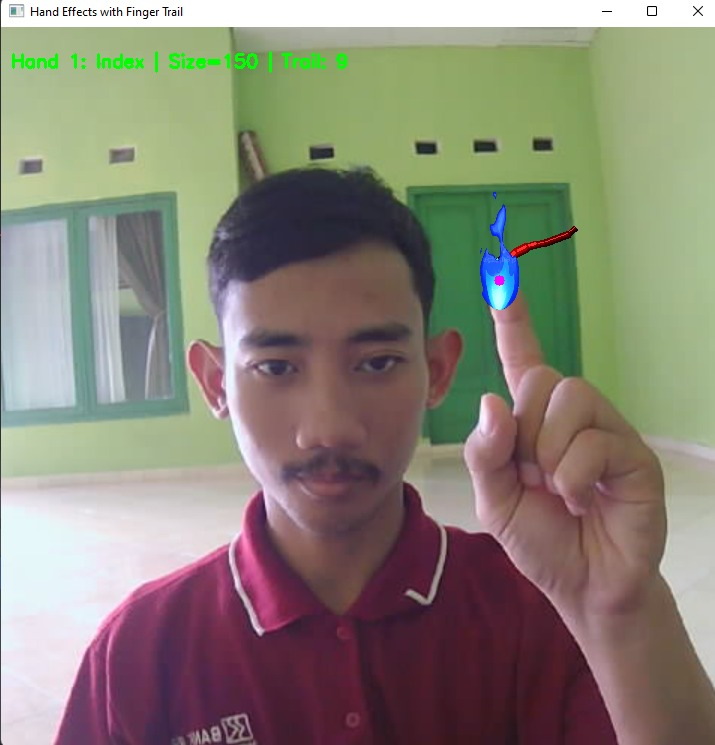
\includegraphics[width=0.5\textwidth]{Figure/one-finger.jpg}
        \caption{Mendeteksi Satu Jari}
        \label{fig:hand_sign_calculator}
    \end{figure}
    Gambar 4.2 menunjukkan keberhasilan sistem dalam mendeteksi dan membedakan gerakan tangan terbuka dan mengepal. Pada kondisi telapak tangan terbuka, sistem berhasil mengenali keberadaan satu tangan dengan lima jari terentang dan menampilkan efek filter “Superpower” secara tepat di area tangan, khususnya mengikuti posisi jari tengah, sesuai logika kode yang mengaktifkan efek saat jumlah jari terdeteksi lebih dari nol. Sebaliknya, saat tangan mengepal, sistem tidak menampilkan efek karena jumlah jari terbuka tidak memenuhi syarat aktivasi, menunjukkan bahwa kode mampu menjalankan klasifikasi gestur secara akurat dan mengeksekusi filter hanya saat kondisi yang sesuai terpenuhi.
    \begin{figure}[H]
        \centering
        \begin{minipage}[b]{0.45\textwidth}
            \centering
            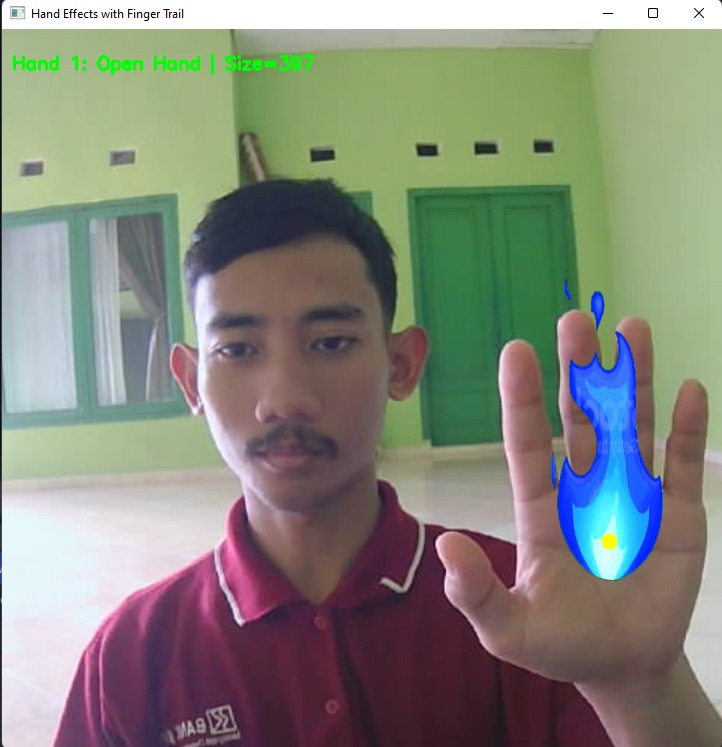
\includegraphics[width=\textwidth]{Figure/telapak.jpg}
            \caption*{(a) Telapak Tangan}
        \end{minipage}
        \hfill
        \begin{minipage}[b]{0.45\textwidth}
            \centering
            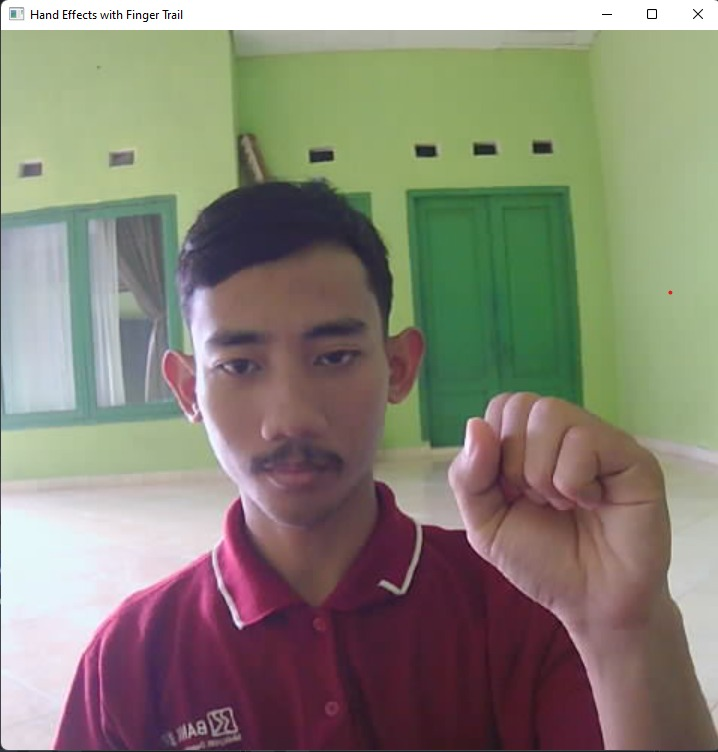
\includegraphics[width=\textwidth]{Figure/mengepal.jpg}
            \caption*{(b) Mengepal}
        \end{minipage}
        \caption{Deteksi Gerakan Tangan}
        \label{fig:telapak_mengepal}
    \end{figure}

    Gambar 4.3 menunjukkan keberhasilan program dalam mendeteksi dua tangan secara real-time, dengan identifikasi gestur berbeda: tangan kiri dikenali sebagai satu jari menunjuk dan tangan kanan sebagai telapak tangan terbuka. Efek visual berupa nyala api biru ditampilkan secara dinamis di atas jari telunjuk dan telapak tangan, menyesuaikan posisi tangan yang terdeteksi. Informasi tambahan seperti ukuran tangan dan panjang jejak (trail) juga ditampilkan sebagai overlay teks.
    \begin{figure}[H]
        \centering
        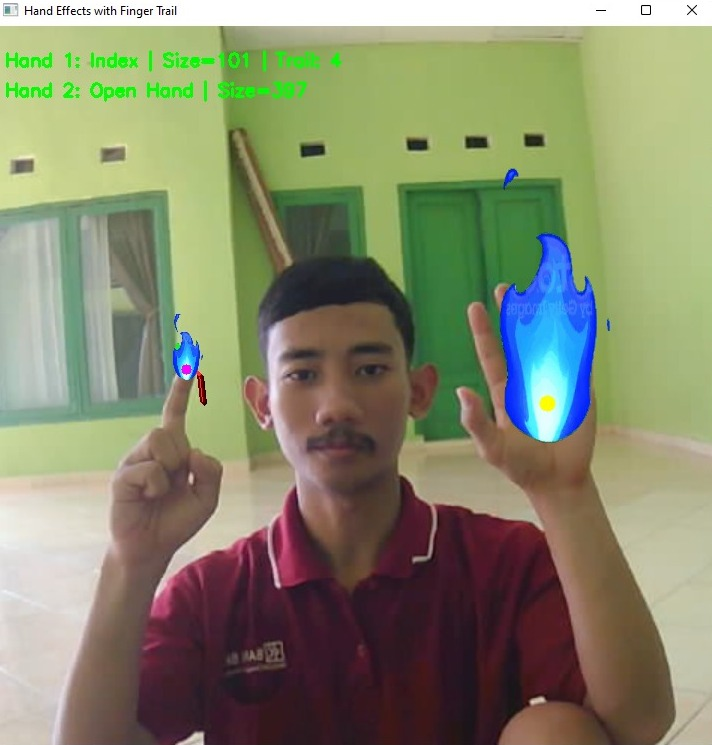
\includegraphics[width=0.5\textwidth]{Figure/double-filter.jpg}
        \caption{Deteksi Satu Jari dan Telapak Tangan}
        \label{fig:number_detection}
    \end{figure}

    \subsection{Pembahasan}

    Program ini mengimplementasikan sistem deteksi landmark tangan berbasis MediaPipe yang mampu mengidentifikasi 21 titik anatomi kunci pada tangan secara real-time melalui webcam. Sistem menggunakan kombinasi OpenCV untuk pengolahan citra, MediaPipe untuk deteksi landmark, dan imageio untuk memuat efek visual berformat GIF. Arsitektur dibagi menjadi beberapa komponen utama yaitu gesture recognition engine yang menganalisis konfigurasi landmark untuk mengenali gesture (fist, open hand, single finger), position smoothing system untuk stabilisasi koordinat menggunakan exponential smoothing, dan visual effects renderer yang menampilkan animasi GIF pada posisi yang ditentukan berdasarkan gesture yang terdeteksi.
    
    Sistem menyediakan tiga mode interaksi utama berdasarkan gesture yang terdeteksi: mode fist untuk reset tracking, mode open hand yang menempatkan efek visual di tengah telapak tangan, dan mode single finger yang menampilkan efek di ujung jari disertai dengan trail berwarna merah yang mengikuti pergerakan fingertip. Implementasi visual menggunakan teknik alpha blending untuk overlay efek GIF dengan transparansi, dynamic sizing berdasarkan ukuran tangan yang terdeteksi, dan trail rendering dengan shadow effect yang memberikan kesan depth. Project ini juga menerapkan optimisasi performa melalui frame resizing, bounds checking untuk overlay operations, dan caching sistem untuk mencegah recomputation yang tidak perlu, sehingga dapat berjalan smooth pada hardware standar dengan frame rate yang stabil.
    

\newpage
\section{Cara Instalasi dan Penggunaan}
    \subsection{Cara Instalasi}
    \begin{itemize}
        \item Clone Repository ini: git clone https://github.com/han5474ni/Tugas-besar-Multimedia
   \item Buat dan Aktifkan Virtual Environment: python -m venv venv
   \begin{itemize}
       \item Windows: ./venv/Scripts/activate
       \item macOS/Linux: source venv/bin/activate
   \end{itemize}
   \item Instal Dependensi: pip install -r requirements.txt
    \end{itemize}
   \subsection{Cara Menggunakan}
    \begin{itemize}
        \item Pastikan webcam terhubung dan berfungsi dengan baik
        \item Jalankan program: python main.py
        \item Kontrol Gestur: Telapak Tangan Terbuka, satu Jari
        \item Kepalan Tangan
        \item ESC atau Q: untuk keluar
    \end{itemize}
    
\newpage
\bibliographystyle{IEEEtran}
\bibliography{Referensi}
\end{document}
